\section{PMOS}
\subsection{Part A}
Using the circuit shown in figure \ref{fig:pmos_circuit} we measured $I_{sd}$ as we varied the drain voltage from within the range of $0 V \le V_{sd} \le 5 V$. 
The value of the gate voltage was set to $V_{sg} = 2.5V$. 
\\

\FloatBarrier

\begin{figure}[h!]
	\centering
	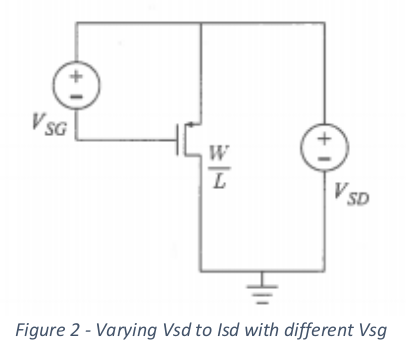
\includegraphics[scale=0.75]{../images/pmos_circuit}
	\caption{The PMOS transistor circuit used for our measurements.}
	\label{fig:pmos_circuit}
\end{figure}

\FloatBarrier
We can see from the $I_{sd}$ vs $V_{sd}$ curve in figure \ref{fig:pmos} that this PMOS transistor is in cutoff until $V_{sd} \approx 1.8 V$. 

\FloatBarrier

\begin{figure}[h!]
	\centering
	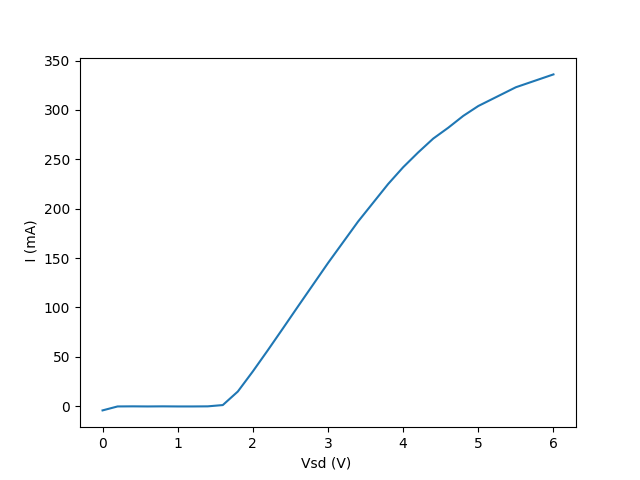
\includegraphics[scale=0.75]{../data/pmos.png}
	\caption{The resulting $I_{sd}$ vs $V_{sd}$ graph for $V_{sg}=2.5V$}
	\label{fig:pmos}
\end{figure}

\FloatBarrier
To turn on this transistor the gate voltage must be less than the source voltage by at least the absolute value of the threshold voltage. 
This means that at $V_{sd} = 1.8 V$, $V_{sg} \le |V_{tp}|$.
\\
To operate in triode mode the drain voltage must be greater than the gate voltage by at least the absolute value of the threshold voltage.
The transistor enters triode mode at $ V_{sd} \le 1.8V$.
Given that our data did not show signs of entering saturation mode, we were unable to find the saturation edge.
\subsection{Part B}
For part B we used the procedures from part A, but changed the gate voltage to $V_{sg} = 5 V$. 

\FloatBarrier

\begin{figure}[h!]
	\centering
	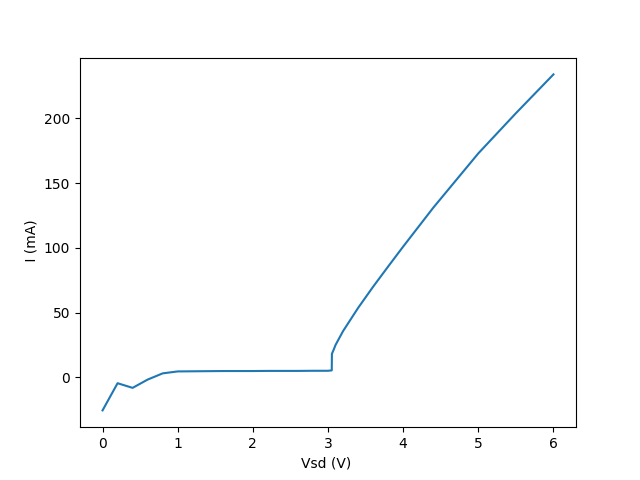
\includegraphics[scale=0.75]{../data/pmos_5v.png}
	\caption{The resulting $I_{sd}$ vs $V_{sd}$ graph for $V_{sg}=5V$}
	\label{fig:pmos_5v}
\end{figure}

\FloatBarrier
We see that the transistor operates in cutoff until $V_{sd} = 3.05 V$.
The difference in $V_{sd}$ from part A has to do with the fixed gate voltage and the variable drain voltage being connected to the same node at the source.
It then operates in triode mode for the rest of the values we tested up to $V_{sd}=6V$.
Given that our data did not show signs of entering saturation mode, we were unable to find the saturation edge.
